% Created November 2014 by Carl D. Sorensen

\documentclass[letterpaper, 11pt, twoside, article]{memoir}

\setstocksize{11in}{8.5in}
\setlrmarginsandblock{1.5in}{1in}{*}

\setulmarginsandblock{1in}{1in}{*}

\setulmarginsandblock{1in}{1.5in}{*}
\setlength{\footskip}{.5in}

\checkandfixthelayout[classic]

\usepackage[T1]{fontenc}

\usepackage{fontspec}
\usepackage{graphicx}
\usepackage{booktabs}
\usepackage{enumitem}
\usepackage{xcolor, colortbl}
\usepackage{array}
\usepackage{calc}
\usepackage[font=small,singlelinecheck=false]{caption}
\usepackage{pdfpages}
\usepackage{tikz}
\usetikzlibrary{matrix, positioning}




% Template name and version commands
\newcommand{\templateTitle}{ConceptDefinitionTemplate.tex}
\newcommand{\templateRev}{C}
\newcommand{\templateRevDate}{13 Dec 2018}
\newcommand{\templateOwner}{CDS}

% Artifact Identification Information
\newcommand{\artifactID}{CD-XXX}
\newcommand{\artifactTitle}{Artifact Title}
\newcommand{\artifactRev}{Rev}
\newcommand{\artifactDate}{Date}
\newcommand{\artifactPreparer}{Preparer Name(s)}
\newcommand{\artifactChecker}{Checker Name(s)}
\newcommand{\teamName}{Capstone Team Name}


%% Optima is available on a Macintosh; Windows font names will need to be different
%% You will probably need to typeset with XeLaTeX.

\setmainfont[Ligatures=TeX]{Optima} 




%%%%% adjust spacing -- Choose one line to uncomment

%\abnormalparskip{0.5\baselineskip}  %adjusts spacing between paragraphs under user control
\nonzeroparskip  % Default value for non-zero spacing between paragraphs
%\traditionalparskip  % No extra spacing between paragraphs -- recommended by Wilson, the author of the memoir class



% Trick for fixed-width table columns
\newcolumntype{L}[1]{>{\raggedright\let\newline\\\arraybackslash\hspace{0pt}}p{#1}}
\newcolumntype{C}[1]{>{\centering\let\newline\\\arraybackslash\hspace{0pt}}p{#1}}
\newcolumntype{R}[1]{>{\raggedleft\let\newline\\\arraybackslash\hspace{0pt}}p{#1}}

% Page Style
\newcommand{\artFoot}{\artifactID \quad Rev \artifactRev \quad \artifactDate}
\makepagestyle{artifact}
   \makeevenfoot{artifact}{\thepage}{}{\artFoot}
   \makeoddfoot{artifact}{\artFoot}{}{\thepage}

%%% Artifact Header Command -- You shouldn't need to adjust this (unless you want to change the number
%         of rows in the header
\newcommand{\artifactHeader}{
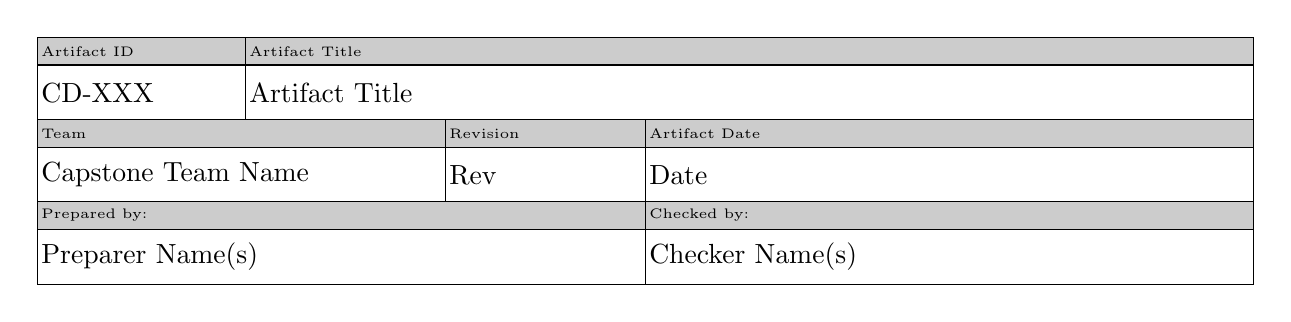
\begin{tikzpicture}
[cell/.style={rectangle,draw=black, inner sep = .5mm},
space/.style={minimum height=1.5em,matrix of nodes,row sep=-\pgflinewidth,column sep=-\pgflinewidth},
every odd row/.style = { nodes={cell,fill=gray!40, anchor = west}, minimum height = 3.5mm, font = \tiny},
every even row/.style = {nodes = {cell, anchor = west},minimum height = 7mm, font = \normalsize },
ampersand replacement = \&,
nodes in empty cells]

\matrix (first) [space, 
column 1/.style={ text width = 1in},
column 2/.style={ text width=5in},
]{
Artifact ID \& Artifact Title \\
\artifactID \& \artifactTitle \\
};
\matrix (second) [space, below = -2.7mm of first,
column 1/.style={ text width = 2in},
column 2/.style={ text width=1in-1mm},
column 3/.style={text width = 3in}
]
{
Team \& Revision \& Artifact Date \\
\teamName \& \artifactRev \& \artifactDate \\
};
\matrix (third) [space, below = -2.7mm of second,
column 1/.style={ text width = 3in},
column 2/.style={ text width=3in},
]
{
Prepared by: \& Checked by: \\
\artifactPreparer \& \artifactChecker \\
};
\end{tikzpicture}
}


%%%% BEGINNING OF DOCUMENT
%  Put your document body here

\begin{document}

\pagestyle{artifact}

\raggedright

\artifactHeader

\chapter{Revision History}

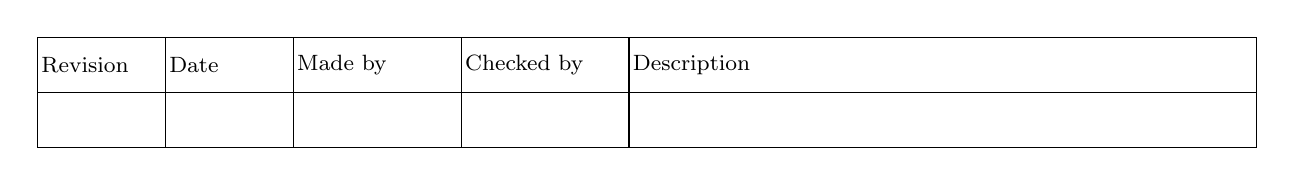
\begin{tikzpicture}
[cell/.style={rectangle,draw=black, inner sep = .5mm, anchor=west, minimum height = 7mm, font=\footnotesize,},
space/.style={matrix of nodes,row sep=-\pgflinewidth,column sep=-\pgflinewidth},
nodes in empty cells]

\matrix (first) [space, 
column 1/.style={nodes={cell, text width = .6 in}},
column 2/.style={ nodes={cell, text width = .6 in}},
column 3/.style={ nodes={cell, text width = .8 in}},
column 4/.style={ nodes={cell, text width = .8 in}},
column 5/.style={ nodes={cell, text width = 3.1 in}},
]{
Revision & Date & Made by & Checked by & Description \\
& & & & \\  %add new lines here for each revision
};
\end{tikzpicture}

\chapter{References}

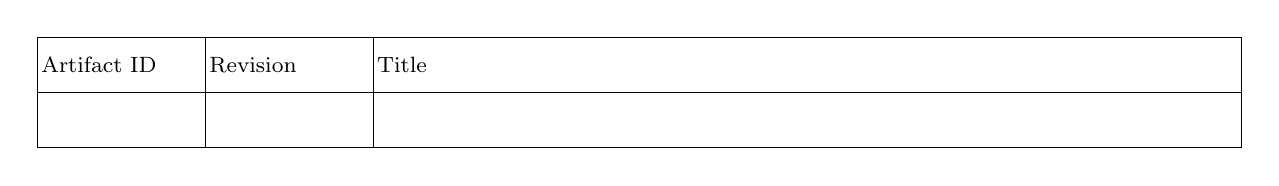
\begin{tikzpicture}
[cell/.style={rectangle,draw=black, inner sep = .5mm, anchor=west, minimum height = 7mm, font=\footnotesize,},
space/.style={matrix of nodes,row sep=-\pgflinewidth,column sep=-\pgflinewidth},
nodes in empty cells]

\matrix (first) [space, 
column 1/.style={nodes={cell, text width = .8 in}},
column 2/.style={ nodes={cell, text width = .8 in}},
column 3/.style={ nodes={cell, text width = 4.3 in}},
]{
Artifact ID & Revision & Title \\
& & \\  % add new lines here for each reference
};
\end{tikzpicture}

Include references in this table that are needed for the artifact.  This may include one or more computer files.
Remove this paragraph when you create the artifact.

\chapter{Purpose}
Describe the purpose of the artifact, which includes the goal of clearly communicating the concept.

\chapter{Concept Definition}
Use both graphics and words as necessary to clearly communicate the concept.  Remember the concept must
be defined well enough that feasibility, weight, and cost estimates can be made.
 
\chapter{test}
\end{document}
